\documentclass[tikz,border=2mm]{standalone}
\usetikzlibrary{positioning,fit}
\begin{document}
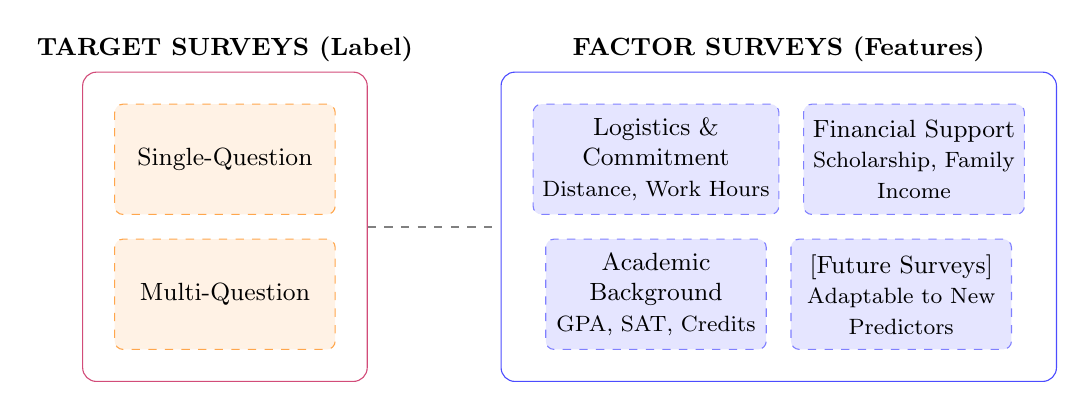
\begin{tikzpicture}[
  box/.style={draw,dashed,rounded corners=3pt,minimum width=28mm,minimum height=14mm,align=center,font=\small},
  target/.style={box,draw=orange!70,fill=orange!10},
  factor/.style={box,draw=blue!50,fill=blue!10},
  container/.style={draw,rounded corners=5pt,inner sep=4mm}
]
% Target surveys
\node[target] (sq) {Single-Question};
\node[target,below=3mm of sq] (mq) {Multi-Question};
\node[container,draw=purple!70,fit=(sq)(mq),label={[font=\small\bfseries]above:TARGET SURVEYS (Label)}] (tbox) {};

% Factor surveys
\node[factor,right=25mm of sq] (lc) {Logistics \&\\Commitment\\{\footnotesize Distance, Work Hours}};
\node[factor,right=3mm of lc] (fs) {Financial Support\\{\footnotesize Scholarship, Family}\\{\footnotesize Income}};
\node[factor,below=3mm of lc] (ab) {Academic\\Background\\{\footnotesize GPA, SAT, Credits}};
\node[factor,right=3mm of ab] (fu) {[Future Surveys]\\{\footnotesize Adaptable to New}\\{\footnotesize Predictors}};
\node[container,draw=blue!70,fit=(lc)(fs)(ab)(fu),label={[font=\small\bfseries]above:FACTOR SURVEYS (Features)}] (fbox) {};

% Connection
\draw[gray,dashed,thick] (tbox.east) -- (fbox.west);
\end{tikzpicture}
\end{document}
